\documentclass[11pt,a4paper]{article}

\usepackage[margin=2.4cm]{geometry}
\usepackage[T1]{fontenc}
\usepackage[utf8]{inputenc}
\usepackage{lmodern}
\usepackage{microtype}
\usepackage{amsmath,amssymb}
\usepackage{graphicx}
\usepackage{booktabs}
\usepackage{multirow}
\usepackage{array}
\usepackage{xcolor}
\usepackage{caption}
\usepackage{enumitem}
\usepackage[colorlinks=true,linkcolor=blue!50!black,citecolor=blue!50!black,urlcolor=blue!50!black]{hyperref}

\graphicspath{{../results/figures/}}
\captionsetup{font=small,labelfont=bf}
\setlist{itemsep=2pt,topsep=4pt}

\newcommand{\best}[1]{\textbf{#1}}

\title{\textbf{How Much 3D Geometry Does a Graph Neural Network Need?}\\[4pt]
\large A controlled study of geometric information in molecular property prediction on QM9}
\author{Manuel Rodr\'iguez Villegas}
\date{October 2026}

\begin{document}
\maketitle

\begin{abstract}
\noindent
We study how much, and which kind, of three-dimensional geometric information helps graph
neural networks predict quantum-chemical properties of small molecules. Five models form a
ladder in which each step adds exactly one ingredient: topology only (GIN), bond types
(GINEdge), bond lengths (GINDist), an EGNN-style network with the same information
(EGNNStatic), and E(3)-equivariant coordinate updates (EGNN). All models share the training
protocol and a parameter budget of $\sim$200k, and are trained with three seeds on four QM9
targets. Equivariant coordinate updates give the largest single improvement ($-32\%$ error
against their exact control), concentrated on the dipole moment ($-41\%$), the most
direction-dependent property. An inference-time noise ablation shows that models trained
on exact DFT geometries are extremely brittle: a perturbation of $0.05$\,\AA{} makes every
geometric model worse than the topology-only baseline. Retraining with noise of the same
size separates the two geometric models: the distance-based GINDist loses its entire
advantage, revealing that it exploited sub-$0.05$\,\AA{} precision, while EGNN keeps its
accuracy and becomes $7\times$ more robust. Finally, an Ollivier--Ricci curvature analysis
finds at most a weak over-squashing signal, and shows that on molecular graphs with explicit
hydrogens the curvature mostly measures hybridisation rather than topological bottlenecks.
\end{abstract}

% ---------------------------------------------------------------------------------------
\section{Introduction}

Predicting molecular properties with machine learning replaces expensive quantum-chemical
calculations (density functional theory, DFT: minutes to hours per molecule) with
millisecond inference, which makes screening of large chemical spaces feasible. Graph neural
networks (GNNs) are the standard tool: atoms are nodes, bonds are edges, and information is
exchanged between neighbouring atoms by message passing~\cite{gilmer2017}.

A molecule, however, is not only a graph: it has a 3D geometry, and most physical properties
depend on it. A central design question is therefore \emph{how} a network should use the
coordinates. Using them naively breaks a fundamental symmetry: rotating or translating a
molecule does not change its properties, so predictions must be invariant to the Euclidean
group E(3). Two families of solutions exist: models that only read invariant quantities such
as interatomic distances~\cite{schutt2017}, and equivariant models whose internal geometric
representations rotate with the input~\cite{satorras2021}.

This project asks a deliberately narrow question: \emph{which geometric ingredient brings
which improvement, and why?} Rather than chasing benchmark numbers, the experiments are
designed so that every comparison isolates one variable. The contributions are:
\begin{enumerate}
  \item A five-model ladder with matched parameter counts, identical training and three
        seeds, in which each adjacent pair differs in a single ingredient (Section~\ref{sec:setup}).
  \item Evidence that equivariant coordinate updates are the most valuable ingredient on a
        bond graph, with gains graded by target as physics suggests (Section~\ref{sec:main}).
  \item A noise ablation and a noise-augmented retraining that distinguish models that learn
        geometric \emph{structure} from models that memorise geometric \emph{precision}
        (Sections~\ref{sec:noise} and~\ref{sec:augmentation}).
  \item An over-squashing analysis with Ollivier--Ricci curvature, controlled for molecule
        size, and the observation that explicit hydrogens turn curvature into a proxy for
        hybridisation (Section~\ref{sec:curvature}).
\end{enumerate}

% ---------------------------------------------------------------------------------------
\section{Background}

\paragraph{Message passing.} A message-passing network updates each node embedding $h_i$
from its neighbours $\mathcal{N}(i)$:
$h_i^{(l+1)} = \phi\big(h_i^{(l)}, \textstyle\sum_{j\in\mathcal{N}(i)} \psi(h_i^{(l)}, h_j^{(l)}, e_{ij})\big)$,
and a permutation-invariant readout pools node embeddings into a graph prediction. With $L$
layers, each node sees its $L$-hop neighbourhood. The Graph Isomorphism Network
(GIN)~\cite{xu2019} uses sum aggregation and an MLP update, which makes it as expressive as
the 1-Weisfeiler--Lehman test, the upper bound for this family. It is therefore a strong,
honest baseline: any gain of a geometric model over GIN cannot be blamed on a weak baseline.

\paragraph{Invariance and equivariance.} A function $f$ is invariant to a group $G$ if
$f(g\cdot x)=f(x)$ and equivariant if $f(g\cdot x) = g\cdot f(x)$. Scalar molecular
properties must be E(3)-invariant. Distances $\|x_i-x_j\|$ are invariant, so any network that
only reads distances is invariant by construction. Note that a model that ignores the
coordinates altogether, such as GIN, is also invariant, trivially: invariance is easy;
being invariant \emph{and} geometry-aware is the problem.

\paragraph{EGNN.} The E(n)-equivariant GNN of Satorras et al.~\cite{satorras2021} updates
both node features and coordinates. For an edge $j\to i$,
\begin{align}
  m_{ij} &= \phi_e\big(h_i, h_j, \|x_i-x_j\|, a_{ij}\big), \qquad
  h_i' = h_i + \phi_h\Big(h_i, \textstyle\sum_{j} m_{ij}\Big), \\
  x_i' &= x_i + \frac{1}{|\mathcal{N}(i)|}\sum_{j\in\mathcal{N}(i)} \frac{x_i-x_j}{\|x_i-x_j\|+1}\,\phi_x(m_{ij}).
\end{align}
Messages depend only on invariants, so $h$ stays invariant; coordinates move only along
relative position vectors scaled by invariant scalars, so $x$ is equivariant. Reading out
from $h$ alone yields invariant predictions. Because later layers compute distances between
\emph{updated} positions, which depend on the positions of neighbours of neighbours, the
network gains access to bond and dihedral angles even though every message only sees
distances. On a bond graph, this is the only route to angular information.

\paragraph{Over-squashing and curvature.} Information from an exponentially growing
receptive field must pass through fixed-size vectors; bottlenecks in the graph aggravate this
over-squashing~\cite{alon2021}. Topping et al.~\cite{topping2022} linked bottlenecks to
negatively curved edges. We use the Ollivier--Ricci curvature~\cite{ollivier2009}
$\kappa(u,v) = 1 - W_1(\mu_u,\mu_v)$, where $\mu_x$ is the lazy random walk at $x$ (mass
$\alpha=\tfrac12$ on $x$, the rest spread uniformly over its neighbours) and $W_1$ is the
Wasserstein-1 distance under the shortest-path metric. Positive curvature indicates dense,
clique-like neighbourhoods; negative curvature indicates bridges.

% ---------------------------------------------------------------------------------------
\section{Experimental setup}\label{sec:setup}

\paragraph{Data.} QM9~\cite{ramakrishnan2014} contains 130{,}831 small organic molecules
(up to 9 heavy atoms among C, N, O, F; up to 29 atoms with hydrogens) with DFT-relaxed
geometries (B3LYP/6-31G(2df,p)). Four targets were chosen to span different physics
(Table~\ref{tab:targets}). The data are split at random into 110{,}000 / 10{,}000 / 10{,}831
molecules with a fixed seed, shared by every model and training seed. A random split matters:
QM9 is stored in enumeration order, and a contiguous split (as in an earlier version of this
project) gives a test set of systematically different molecules (mean of 15.8 atoms against
18.0 in training). Targets are standardised with training-set statistics only, so the
multi-task loss weighs all targets equally.

\begin{table}[h]
\centering
\small
\setlength{\tabcolsep}{4pt}
\begin{tabular}{llllc}
\toprule
Target & Property & Unit & Physical origin & Extensive? \\
\midrule
$\mu$      & dipole moment (norm)        & D            & $\sum_i q_i \mathbf{r}_i$, charge-weighted positions & no (vector sum) \\
$\alpha$   & isotropic polarisability    & $a_0^3$      & deformability of the electron cloud & yes \\
gap        & HOMO--LUMO gap              & eV           & frontier-orbital energies, conjugation & no (intensive) \\
$C_v$      & heat capacity at 298\,K     & cal/(mol\,K) & vibrational modes, bond stiffness & yes \\
\bottomrule
\end{tabular}
\caption{Prediction targets.}
\label{tab:targets}
\end{table}

\paragraph{Models.} All models operate on the covalent-bond graph with explicit hydrogens
and share the same atom embedding, depth (4 layers, residual connections, SiLU activations)
and readout. They differ only in their encoder (Table~\ref{tab:models}):
\begin{itemize}
  \item \textbf{GIN}: GINConv layers; ignores bond types and coordinates.
  \item \textbf{GINEdge}: GINEConv~\cite{hu2020} layers with an MLP encoding of the bond type.
  \item \textbf{GINDist}: as GINEdge, with the bond length added to the edge features.
  \item \textbf{EGNNStatic}: EGNN layers with coordinate updates disabled. It reads exactly
        the same information as GINDist (bond type and bond length) through a different
        architecture.
  \item \textbf{EGNN}: EGNN layers with equivariant coordinate updates.
\end{itemize}
Distances are expanded on 32 Gaussian radial basis functions between 0 and 5\,\AA{}, as in
SchNet~\cite{schutt2017}, identically for the three distance-aware models. The readout
concatenates sum and mean pooling (sum suits extensive properties, mean intensive ones) and
feeds one small MLP head per target on top of the shared trunk. Hidden sizes were chosen so
that every model has $\sim$200k parameters (within $\pm1.5\%$); at equal width EGNN would
have $2.7\times$ more parameters than GIN, and any gain could be attributed to capacity.

\begin{table}[h]
\centering
\small
\begin{tabular}{lcccccc}
\toprule
Model & Bond types & Distances & Coord.\ updates & Hidden & Parameters & Hours/run \\
\midrule
GIN        & --         & --         & --         & 128 & 200.7k & 0.87 \\
GINEdge    & \checkmark & --         & --         & 122 & 198.1k & 0.89 \\
GINDist    & \checkmark & \checkmark & --         & 122 & 202.0k & 0.92 \\
EGNNStatic & \checkmark & \checkmark & --         & 82  & 202.7k & 1.02 \\
EGNN       & \checkmark & \checkmark & \checkmark & 76  & 198.8k & 1.18 \\
\bottomrule
\end{tabular}
\caption{The model ladder. All models read atom types and the bond graph. Training time per
run on one NVIDIA H200 MIG slice (1g.18gb).}
\label{tab:models}
\end{table}

\paragraph{Training.} All models use the same protocol: Adam (learning rate
$5\times10^{-4}$), cosine annealing over 300 epochs, batch size 96, L1 loss in normalised
units, gradient clipping at norm 10, and early stopping with patience 50 on validation MAE.
The checkpoint with the best validation MAE is restored before testing. Each model is trained
with three seeds; we report mean $\pm$ standard deviation.

\paragraph{Correctness checks.} A test suite verifies, in double precision and to $10^{-9}$,
that every model's predictions are invariant to rotations, reflections, translations and
atom permutations; that EGNN's output coordinates are equivariant; that GIN and GINEdge do
not depend on coordinates at all; and that curvature values match hand-computed cases.

% ---------------------------------------------------------------------------------------
\section{Results}

\subsection{Main comparison}\label{sec:main}

\begin{table}[t]
\centering
\small
\setlength{\tabcolsep}{4pt}
\begin{tabular}{lccccc}
\toprule
Model & Combined (norm.) & $\mu$ [D] & $\alpha$ [$a_0^3$] & gap [eV] & $C_v$ [cal/mol/K] \\
\midrule
GIN        & $0.1094 \pm 0.0002$ & $0.397 \pm 0.002$ & $0.314 \pm 0.001$ & $0.125 \pm 0.001$ & $0.154 \pm 0.001$ \\
GINEdge    & $0.1036 \pm 0.0003$ & $0.379 \pm 0.001$ & $0.302 \pm 0.004$ & $0.117 \pm 0.000$ & $0.142 \pm 0.001$ \\
GINDist    & $0.0756 \pm 0.0011$ & $0.285 \pm 0.005$ & $0.224 \pm 0.002$ & $0.086 \pm 0.001$ & $0.074 \pm 0.001$ \\
EGNNStatic & $0.0825 \pm 0.0011$ & $0.314 \pm 0.004$ & $0.236 \pm 0.005$ & $0.093 \pm 0.001$ & $0.083 \pm 0.002$ \\
EGNN       & \best{0.0559} $\pm$ \best{0.0021} & \best{0.184} $\pm$ 0.011 & \best{0.194} $\pm$ 0.004 & \best{0.079} $\pm$ 0.000 & \best{0.065} $\pm$ 0.001 \\
\bottomrule
\end{tabular}
\caption{Test MAE on clean geometries, mean $\pm$ std over three seeds. The combined score is
the mean of the four MAEs in normalised units (each target has unit variance in training).}
\label{tab:main}
\end{table}

\begin{figure}[t]
\centering
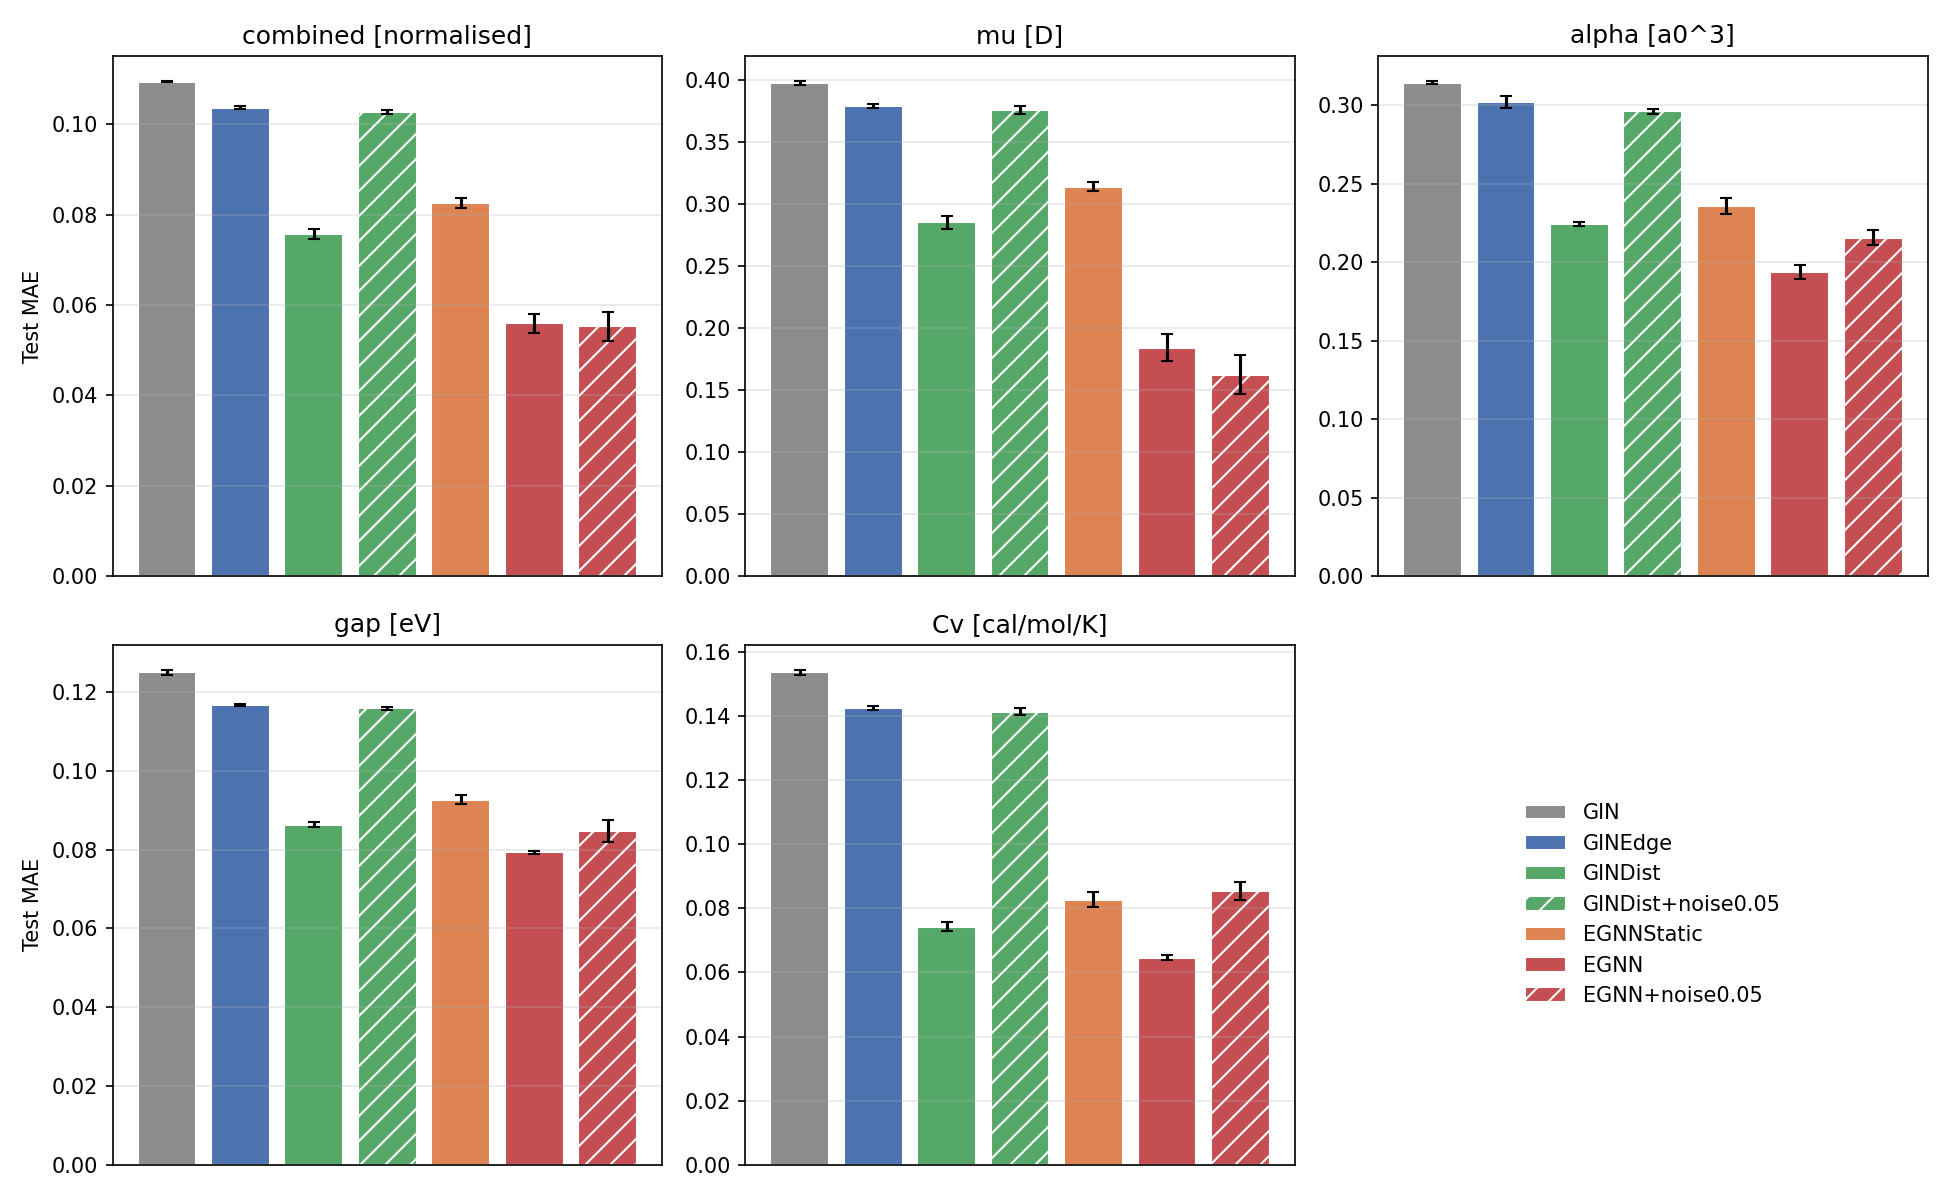
\includegraphics[width=0.95\linewidth]{test_mae.png}
\caption{Test MAE per model (combined in normalised units, targets in physical units).
Hatched bars are the noise-trained variants of Section~\ref{sec:augmentation}.
Error bars: $\pm1$ std over three seeds.}
\label{fig:main}
\end{figure}

Table~\ref{tab:main} and Figure~\ref{fig:main} summarise the comparison. Seed-to-seed
standard deviations are one to two orders of magnitude smaller than the differences between
models, so the ranking is robust. Reading the ladder step by step:

\begin{enumerate}
  \item \textbf{Bond types help a little} (GIN $\to$ GINEdge: $-5\%$). Much of this
        information is already present in the atom features (hybridisation, number of
        attached hydrogens, aromaticity).
  \item \textbf{Bond lengths help a lot} (GINEdge $\to$ GINDist: $-27\%$), most for the
        heat capacity ($-48\%$), which is governed by vibrations and hence by bond
        stiffness, closely related to bond length.
  \item \textbf{With identical information, architecture matters} (GINDist $\to$
        EGNNStatic: $+9\%$, i.e.\ worse). GINDist passes distances through a dedicated edge
        encoder, while EGNN concatenates 32 radial features with two 76-dimensional atom
        embeddings, which dilutes the distance signal. Without the EGNNStatic control, part
        of this architectural difference would have been attributed to equivariance.
  \item \textbf{Equivariant coordinate updates give the largest gain} (EGNNStatic $\to$ EGNN:
        $-32\%$; $-26\%$ against GINDist, $-49\%$ against GIN). The gain is graded by target
        in the order physics suggests (Table~\ref{tab:graded}): largest for the dipole
        moment, a vector sum of charged positions that depends on directions, and smallest
        for the HOMO--LUMO gap, which is dominated by electronic structure (conjugation) and
        is almost topological.
\end{enumerate}

\begin{table}[h]
\centering
\small
\begin{tabular}{lcccc}
\toprule
& $\mu$ & $C_v$ & $\alpha$ & gap \\
\midrule
EGNNStatic $\to$ EGNN (normalised MAE) & $-41\%$ & $-22\%$ & $-18\%$ & $-15\%$ \\
\bottomrule
\end{tabular}
\caption{Effect of equivariant coordinate updates per target, against their exact control.}
\label{tab:graded}
\end{table}

\paragraph{Comparison with the literature.} The original EGNN reports $\mu$: 0.029\,D,
$\alpha$: 0.071\,$a_0^3$, gap: 48\,meV, $C_v$: 0.031\,cal/mol/K~\cite{satorras2021}. Our errors
are $1.6\times$ (gap) to $6\times$ ($\mu$) larger, for documented reasons: a bond graph
instead of a fully connected one (no non-bonded interactions, which matter most for $\mu$), a
single multi-task model of 200k parameters instead of one model per property, and 300 instead
of 1000 epochs. Validation curves were still improving slowly at the end of training (best
epochs between 252 and 294). The goal was a controlled comparison, not a benchmark.

\subsection{Robustness to coordinate noise}\label{sec:noise}

QM9 geometries are DFT energy minima. In practice, such geometries are as expensive as the
properties themselves, and a screening pipeline would use cheaper conformers (force fields,
RDKit) with errors of roughly $0.1$--$0.5$\,\AA{}. We therefore evaluate the trained models on
test geometries perturbed by isotropic Gaussian noise of standard deviation $\sigma$, without
retraining and with the bond graph unchanged. The noise is drawn from seeded generators shared
by all models (paired comparison) and averaged over five realisations.

\begin{figure}[t]
\centering
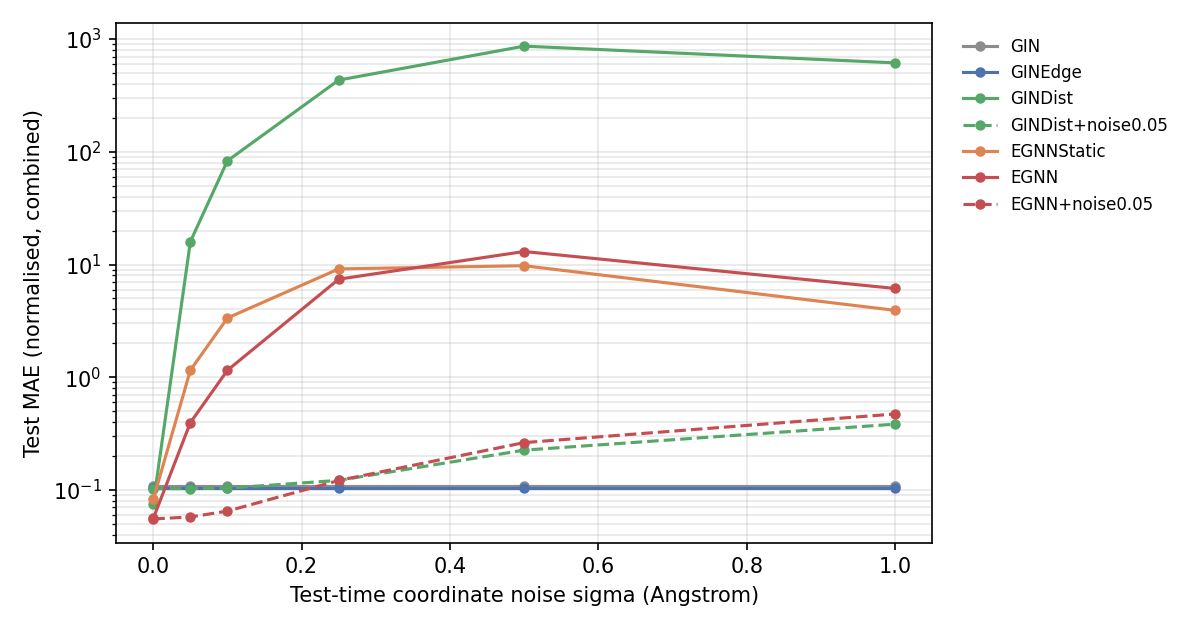
\includegraphics[width=0.85\linewidth]{noise_summary.png}
\caption{Test MAE (combined, log scale) against test-time coordinate noise. Solid: trained on
exact geometries. Dashed: trained with $0.05$\,\AA{} noise (Section~\ref{sec:augmentation}).
GIN and GINEdge ignore coordinates and are exactly flat. The full per-target figure is
\texttt{results/figures/noise\_ablation.png}.}
\label{fig:noise}
\end{figure}

GIN and GINEdge are exactly flat (Figure~\ref{fig:noise}), a built-in sanity check: no
coordinate information leaks into them. Every geometric model, in contrast, collapses: at
$\sigma = 0.05$\,\AA{}, smaller than thermal vibration amplitudes, all of them become
\emph{worse than the topology-only GIN}. GINDist's error grows by a factor of 210, EGNN's by
7, and the seed-to-seed spread becomes as large as the mean, i.e.\ out-of-distribution
behaviour is arbitrary. In QM9, bond lengths of a given type vary very little across molecules (standard
deviation of 0.007\,\AA{} for C--H bonds, 0.009\,\AA{} for C=O and 0.04\,\AA{} for C--C
single bonds), while noise of $\sigma=0.05$\,\AA{} per coordinate changes each bond length
by about $0.07$\,\AA{}. The models learn to read minute distance differences as signal, and
such a perturbation moves them entirely out of the training distribution. GINDist's particularly violent failure is consistent with out-of-distribution
radial features being amplified by batch normalisation, which EGNN does not use; we did not
verify this hypothesis.

\subsection{Training with coordinate noise}\label{sec:augmentation}

To test whether this brittleness is inevitable, we retrained GINDist and EGNN (three seeds
each) with Gaussian noise of $\sigma_{\text{train}} = 0.05$\,\AA{} added to the coordinates of
every training batch, keeping validation and test geometries clean.

\begin{table}[h]
\centering
\small
\begin{tabular}{lccccc}
\toprule
& \multicolumn{5}{c}{Test MAE (combined, normalised) at test-time noise $\sigma$ [\AA]} \\
\cmidrule(lr){2-6}
Model & 0 (clean) & 0.05 & 0.1 & 0.25 & 0.5 \\
\midrule
GIN (reference)          & 0.1094 & 0.1094 & 0.1094 & 0.1094 & 0.1094 \\
GINDist                  & 0.0756 & 15.9   & 83.3   & 433    & 866    \\
GINDist + noise 0.05     & 0.1027 & 0.1028 & 0.1037 & 0.1217 & 0.2256 \\
EGNN                     & 0.0559 & 0.3956 & 1.153  & 7.41   & 13.0   \\
EGNN + noise 0.05        & \best{0.0553} & \best{0.0576} & \best{0.0649} & 0.1213 & 0.2630 \\
\bottomrule
\end{tabular}
\caption{Noise-augmented training. Means over three seeds.}
\label{tab:augmentation}
\end{table}

Table~\ref{tab:augmentation} shows the key result of the project. Noise augmentation makes
both models robust, but it affects their clean accuracy in opposite ways:
\begin{itemize}
  \item \textbf{GINDist loses its whole advantage}: its clean error rises from 0.0756 to
        0.1027, the level of GINEdge (0.1036), the model without distances. Everything
        GINDist gained from distances was therefore precision below $0.05$\,\AA{}, a
        fingerprint of the exact DFT geometry rather than usable geometric information.
  \item \textbf{EGNN keeps its whole advantage}: 0.0553 against 0.0559, within seed
        variation, while becoming $7\times$ more accurate at $\sigma=0.05$\,\AA{} and
        staying better than GIN up to $\sigma\approx0.2$\,\AA{}. What EGNN extracts from the
        geometry (directions and angles, through its coordinate updates) survives
        perturbations that destroy precise bond lengths.
\end{itemize}
The trade-off is target-specific. With noise, EGNN's dipole-moment error \emph{decreases}
by 12\% (noise acts as a regulariser for the most direction-dependent target), whereas the
heat capacity, which depends on precise bond stiffness, degrades by 32\% ($\alpha$: $+11\%$,
gap: $+7\%$). Without this experiment, the two geometric models would have looked like two
degrees of the same thing; with it, they turn out to exploit geometry in qualitatively
different ways.

\subsection{Over-squashing and curvature}\label{sec:curvature}

For every test molecule we compute the Ollivier--Ricci curvature of all edges (exactly, by
solving each small transport problem with POT) and use the minimum edge curvature as a
bottleneck score. Molecules are ranked by it (ties broken by mean curvature) and split into
four equal quantiles, Q0 (least bottlenecked) to Q3 (most). Because larger molecules have both
more negative curvature and different errors, we also regress the per-molecule improvement over
GIN on standardised bottleneck severity, with and without the number of atoms as a covariate.

\paragraph{A hydrogen artefact.} On the all-atom graph, 61\% of test molecules share a minimum
curvature of exactly $-0.5$, and 88\% of those with 19 atoms or more
(Figure~\ref{fig:curvature}, top). The reason is local: for a single bond between two atoms of
degree four, such as the C--C bond of ethane, each walk spreads $1/8$ of its mass on every
neighbour, the surplus $3/8$ crosses the bond, and the three hydrogens of one carbon must
travel three hops to those of the other, so $W_1 = 3/8 + 3\cdot 3/8 = 3/2$ and $\kappa = -1/2$.
On the hydrogen-free skeleton the same bond has $\kappa = +1$. With explicit hydrogens, minimum
curvature therefore measures \emph{saturation} (sp$^3$--sp$^3$ bonds) far more than topological
bottlenecks, and it correlates strongly with size ($r=-0.56$).

\begin{figure}[t]
\centering
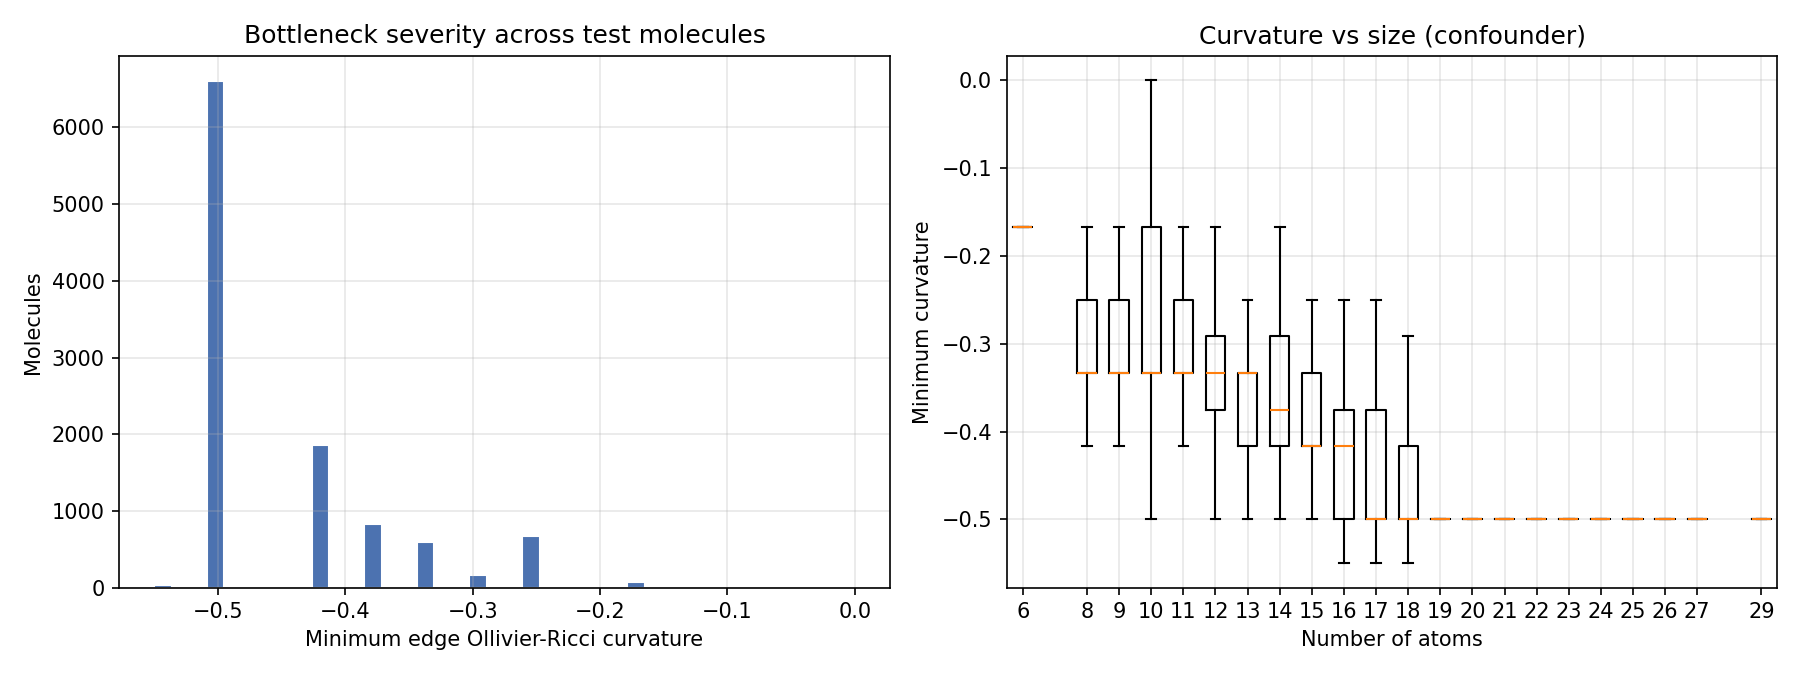
\includegraphics[width=0.82\linewidth]{curvature_distribution.png}\\[2pt]
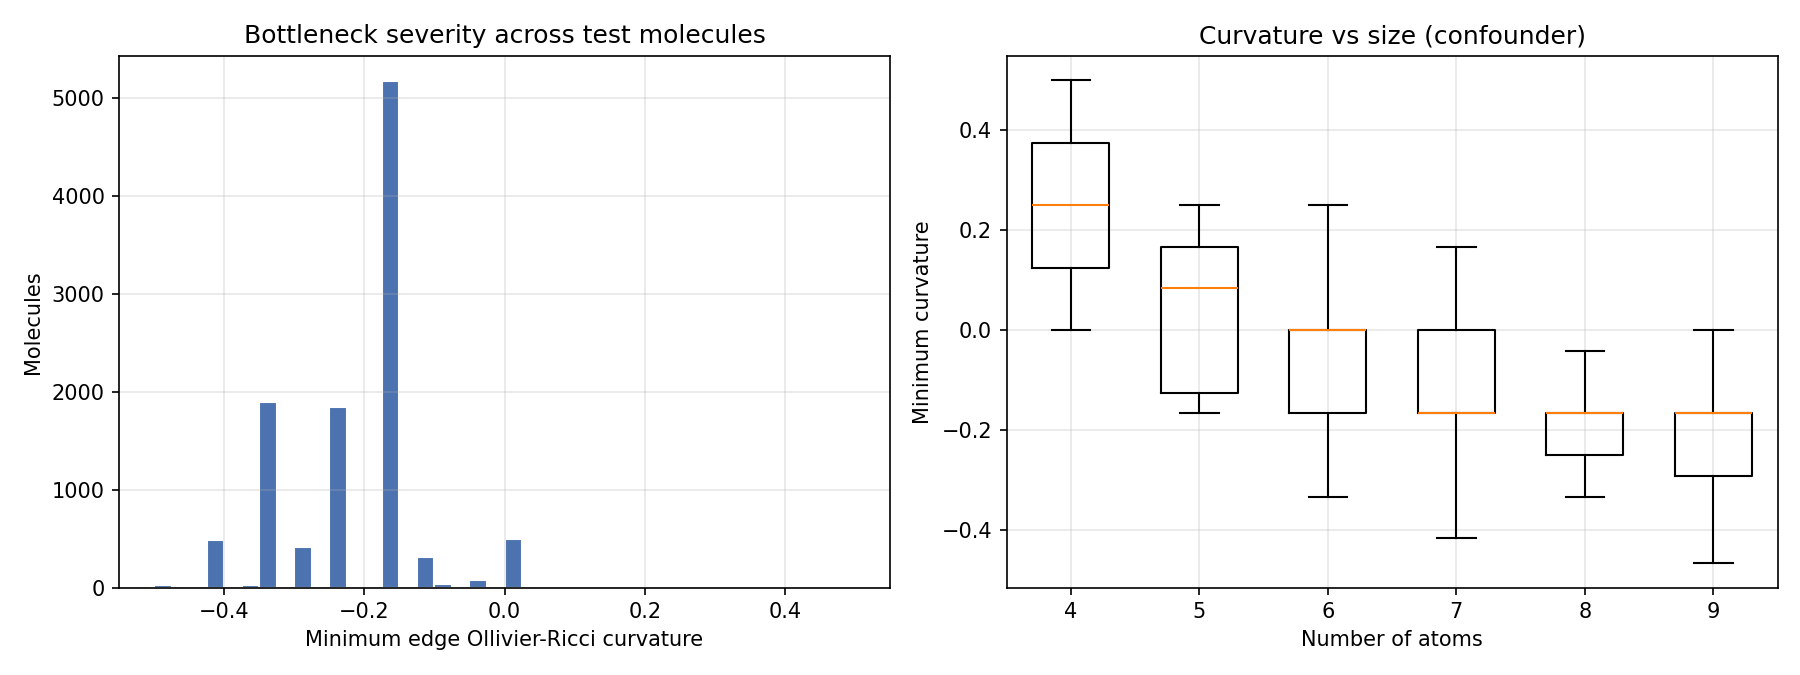
\includegraphics[width=0.82\linewidth]{curvature_distribution_heavy.png}
\caption{Minimum edge curvature per test molecule: histogram (left) and dependence on the
number of nodes (right). Top: all-atom graph, where most molecules sit at exactly $-0.5$ and
curvature tracks size. Bottom: heavy-atom skeleton.}
\label{fig:curvature}
\end{figure}

\paragraph{All-atom graph.} Errors \emph{decrease} with bottleneck severity for every model
(GIN: 0.126 in Q0 to 0.085 in Q3), the opposite of the over-squashing prediction, because Q3
collects larger, saturated, chemically simpler molecules. EGNN's relative gain over GIN rises
mildly (47\% to 51\%), but its absolute per-molecule gain shows no curvature effect once size
is controlled (regression coefficient $-0.0033\pm0.0006$ without size, $-0.0007\pm0.0008$ with
size).

\paragraph{Heavy-atom skeleton.} Removing hydrogens largely removes the size confound
($r=-0.22$; heavy atoms per quantile between 8.6 and 8.9). Now every model's error grows with
bottleneck severity (GIN: $+11\%$ from Q0 to Q3), as over-squashing predicts, and EGNN's
absolute gain over GIN grows slightly but significantly ($+0.0022 \pm 0.0006$ per standard
deviation of severity, after size control). Its relative gain, however, is flat at 47--51\%
(Figure~\ref{fig:improvement}): bottlenecked molecules are harder for every model, but EGNN
does not gain proportionally more on them.

\begin{figure}[t]
\centering
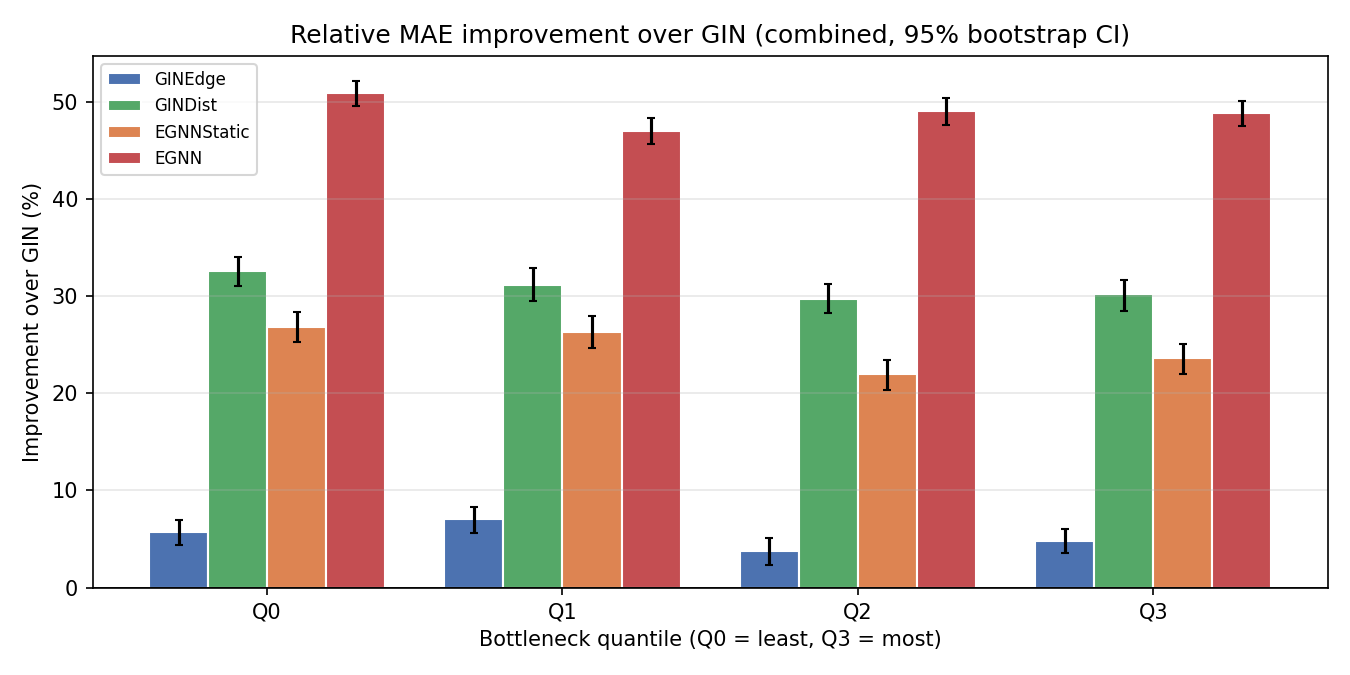
\includegraphics[width=0.75\linewidth]{relative_improvement_by_quantile_heavy.png}
\caption{Relative MAE improvement over GIN per bottleneck quantile on the heavy-atom skeleton,
with paired-bootstrap 95\% confidence intervals.}
\label{fig:improvement}
\end{figure}

Overall, the over-squashing signal is weak at best. This is expected for QM9: molecules have
at most nine heavy atoms and a graph diameter of a few hops, so four message-passing layers
already cover almost the whole molecule, leaving little room for bottlenecks to matter.

% ---------------------------------------------------------------------------------------
\section{Discussion}

\paragraph{What geometry buys, and how to tell.} Clean-data accuracy alone suggests a simple
story, ``more geometry is better''. The controls tell a more precise one. Bond lengths
improve accuracy only as long as the geometry is exact to a few hundredths of an
\AA{}ngstr\"om; equivariant coordinate updates provide information that is robust to such
perturbations and is used where the physics needs directions (the dipole moment). Controls
that hold the information fixed (EGNNStatic) or the noise level fixed (noise-augmented runs)
were necessary to separate these effects.

\paragraph{Accuracy and robustness pull in different directions.} The most accurate models on
DFT geometries were the least robust. For any application where input geometries are
approximate, the relevant model is the noise-trained one, and the relevant evaluation is on
perturbed or generated geometries. Training with noisy coordinates is also the basic ingredient
of denoising pre-training~\cite{zaidi2023} and of 3D diffusion models such as EDM, whose
denoiser is precisely an EGNN~\cite{hoogeboom2022}; these results illustrate why that objective
encourages structural rather than memorised geometric features.

\paragraph{Choosing the symmetry.} All models here are invariant to E(3), which includes
reflections: a chiral molecule and its mirror image receive identical predictions. This is
correct for the scalar properties of isolated molecules in QM9, but wrong whenever a molecule
interacts with a chiral environment, as in nearly every biological setting (proteins are built
from L-amino acids). Such tasks call for SE(3) models or features that change sign under
reflection.

% ---------------------------------------------------------------------------------------
\section{Limitations}

\begin{itemize}
  \item \textbf{Bond graph.} All models use covalent bonds only, which keeps topology
        identical across models and makes the curvature analysis well defined, but ignores
        non-bonded interactions and prevents direct comparison with published numbers.
  \item \textbf{One hyperparameter setting.} The same hyperparameters are used for every model.
        This removes tuning bias but may favour some architectures. Parameters are matched,
        FLOPs are not (EGNN computes edge MLPs).
  \item \textbf{Training length.} Validation error was still decreasing at 300 epochs.
  \item \textbf{Noise model.} Isotropic Gaussian noise produces physically implausible
        geometries; generated conformers would be a more realistic test. Only one training
        noise level ($0.05$\,\AA{}) was explored.
  \item \textbf{Statistics.} Three seeds give reliable rankings here because differences are
        large, but not formal significance tests. The batch-normalisation explanation of
        GINDist's brittleness is an untested hypothesis.
\end{itemize}

% ---------------------------------------------------------------------------------------
\section{Conclusion}

On QM9, with a bond graph, matched capacity and identical training, the most valuable
geometric ingredient is the equivariant coordinate update: it reduces error by a third against
its exact control, most for the dipole moment, and its benefit survives training with
coordinate noise. Distance features also help on clean data, but in this setting their benefit
comes entirely from sub-$0.05$\,\AA{} precision and vanishes once the model must tolerate
realistic geometric error. Models trained on exact geometries are not usable on approximate ones
without noise-aware training. Over-squashing plays at most a minor role in molecules as small as
those in QM9, and with explicit hydrogens Ollivier--Ricci curvature mostly reflects
hybridisation. Natural next steps are a sweep over training noise levels, evaluation on
generated conformers, and the curvature study on larger molecules such as peptides or RNA,
where graph diameters are large enough for bottlenecks to matter.

\paragraph{Reproducibility.} Code, configuration, per-run metrics, training curves and figures
are in the repository. The command \texttt{python main.py all -{}-smoke} runs the full
pipeline on a small subset in about a minute, and \texttt{scripts/dgx\_train.sh} reproduces
all runs on GPUs with Docker.

% ---------------------------------------------------------------------------------------
\begin{thebibliography}{99}
\small
\bibitem{alon2021} U.~Alon and E.~Yahav. On the bottleneck of graph neural networks and its practical implications. \emph{ICLR}, 2021.
\bibitem{gilmer2017} J.~Gilmer, S.~S.~Schoenholz, P.~F.~Riley, O.~Vinyals and G.~E.~Dahl. Neural message passing for quantum chemistry. \emph{ICML}, 2017.
\bibitem{hoogeboom2022} E.~Hoogeboom, V.~G.~Satorras, C.~Vignac and M.~Welling. Equivariant diffusion for molecule generation in 3D. \emph{ICML}, 2022.
\bibitem{hu2020} W.~Hu, B.~Liu, J.~Gomes, M.~Zitnik, P.~Liang, V.~Pande and J.~Leskovec. Strategies for pre-training graph neural networks. \emph{ICLR}, 2020.
\bibitem{ollivier2009} Y.~Ollivier. Ricci curvature of Markov chains on metric spaces. \emph{Journal of Functional Analysis}, 256(3):810--864, 2009.
\bibitem{ramakrishnan2014} R.~Ramakrishnan, P.~O.~Dral, M.~Rupp and O.~A.~von~Lilienfeld. Quantum chemistry structures and properties of 134 kilo molecules. \emph{Scientific Data}, 1:140022, 2014.
\bibitem{satorras2021} V.~G.~Satorras, E.~Hoogeboom and M.~Welling. E($n$) equivariant graph neural networks. \emph{ICML}, 2021.
\bibitem{schutt2017} K.~T.~Sch\"utt, P.-J.~Kindermans, H.~E.~Sauceda, S.~Chmiela, A.~Tkatchenko and K.-R.~M\"uller. SchNet: a continuous-filter convolutional neural network for modeling quantum interactions. \emph{NeurIPS}, 2017.
\bibitem{topping2022} J.~Topping, F.~Di~Giovanni, B.~P.~Chamberlain, X.~Dong and M.~M.~Bronstein. Understanding over-squashing and bottlenecks on graphs via curvature. \emph{ICLR}, 2022.
\bibitem{xu2019} K.~Xu, W.~Hu, J.~Leskovec and S.~Jegelka. How powerful are graph neural networks? \emph{ICLR}, 2019.
\bibitem{zaidi2023} S.~Zaidi, M.~Schaarschmidt, J.~Martens, H.~Kim, Y.~W.~Teh, A.~Sanchez-Gonzalez, P.~Battaglia, R.~Pascanu and J.~Godwin. Pre-training via denoising for molecular property prediction. \emph{ICLR}, 2023.
\end{thebibliography}

\end{document}
